\section{Typisches Aussehen einer Evolutionsstrategie}
%1. Obwohl viel Variation, erkannte Rechenberg Abschnitte die häufig wiederzufinden sind
Evolutionsstrategien weisen einen sehr hohen Grad an Variation auf. Je nach Aufgabengebiet können sich die Verfahren stark unterscheiden.
Rechenberg konnte allerdings Verfahrensabschnitte benennen, aus denen sich typischerweise Evolutionsstrategien zusammensetzen.
Diese Verfahrensabschnitte bilden die Rechenbergsche Grafik-Notation. Diese Notation orientiert sich an Spielkarten und kommt mit lediglich 10 verschiedenen Symbolen aus.
Die gesamte Rechenbergsche Grafik-Notation ist in Abbildung \ref{fig:rechenberg} zu sehen. Abläufe, die in einer natürlichen Evolution stattfinden, finden sich in dieser Notation wieder.
Die Komplexität der Evolutionsstrategien wird durch deren Kombination erreicht.
%2. Die Rechenbergnotation erklären
Die grundlegende Einheit in dieser Notation ist, wie auch schon bei der Codierung, das Individuum. Dieses wird mit einer Spielkarte symbolisiert \ref{fig:individuum}. Die schwarzen Punkte auf der Karte sollen dabei die Chromosomen darstellen.
Eine Population setzt sich aus mehreren Individuen zusammen. Daher wählte Rechenberg einen Stapel \ref{fig:population} an Spielkarten für dessen Darstellung. Zur Verarbeitung der Individuen und der Populationen definierte Rechenberg acht weitere Symbole.
Zum einen muss es für die Verarbeitung von Populationen Methoden geben, mit denen eine Teilmenge an Individuen ausgewählt werden können. Dazu gibt es die gleichverteile Auswahl \ref{fig:auswahl_gleichverteilt} und die Auswahl nach einer Qualitätsfunktion \ref{fig:auswahl_qualitaetsfunktion}.
Der Kreis um die Population soll eine Urne symbolisieren. Bei der gleichverteilten Auwahl hat jedes Individuum die gleiche Wahrscheinlichkeit aus der Urne gezogen zu werden. Bei der Auswahl nach einer Qualitätsfunktion, entscheidet die Qualität der Individuen über die Wahrscheinlichkeit, dass diese Ausgwählt werden.
Je höher die Qualität des Individuum, desto höher die Wahrscheinlichkeit. Auch das Verwenden von isolierten Populationen ist mit der Rechnbergschen Grafik-Notation möglich. Dafür gibt das Populationssymbol \ref{fig:population_isoliert}, welches mit einem Stacheldraht eingegrenzt ist. Dieses Symbol kann hilfreich sein, wenn man mehrere voneinander isolierte Populationen erstellen will, welche sich unabhängig voneinander entwickeln sollen. Alle weiteren Notationssymbole sind Funktionen, die auf einzelne Individuen angewendet werden. Um ein Individuum zu duplizieren, wird das Symbol \ref{fig:duplikation} verwendet. Soll das duplizierte Individuum mutieren, so ist das Symbol \ref{fig:mutation} zu verwenden. Zeigt wie auf dem Symbol \ref{fig:bewertung} ein Pfeil mit einem Q auf ein Individuum, so zeigt das die Anwendung einer Qualitätsfunktion auf das Individuum. Damit auch die Fortpflanzung mehrerer Individuen zu einem neuen Individuum möglich ist, gibt es eigens das Notationssymbol \ref{fig:rekombination} für die Rekombination. Rekombination bedeutet, dass die eine Kombination der Elternchromosome ein neues Kindindividuum erzeugen.
Es kann auch notwendig sein, die genotypischen Merkmale in phänotypische Merkmale umzuwandeln. Dies ist dann notwendig, wenn über die Geninformationen nicht direkt eine Aussage über die Qualität des Individuums getroffen werden kann. In diesen Fällen müssen die Merkmale, die sich aus den Geninformationen ergeben in einer Funktion berechnet werden. Dieses Umwandeln wird mit dem Symbol der phänotypischen Realisation \ref{fig:phaenotypische_realisation} dargstellt.

\begin{figure}
\begin{subfigure}{.3\textwidth}
	\centering
	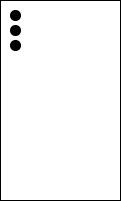
\includegraphics[width=.4\linewidth]{img/rechenberg_notation/individuum.png}
	\caption{Individuum}
	\label{fig:individuum}
\end{subfigure}
\begin{subfigure}{.3\textwidth}
	\centering
	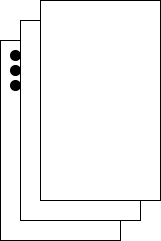
\includegraphics[width=.5\linewidth]{img/rechenberg_notation/population.png}
	\caption{Population}
	\label{fig:population}
\end{subfigure}
\begin{subfigure}{.3\textwidth}
	\centering
	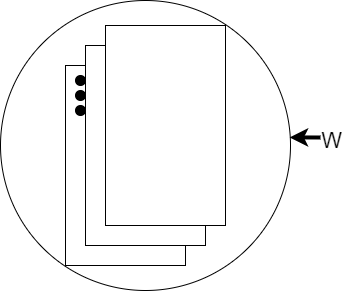
\includegraphics[width=.7\linewidth]{img/rechenberg_notation/auswahl_gleichverteilt.png}
	\caption{Gleichverteilte Auswahl}
	\label{fig:auswahl_gleichverteilt}
\end{subfigure}

\begin{subfigure}{.3\textwidth}
	\centering
	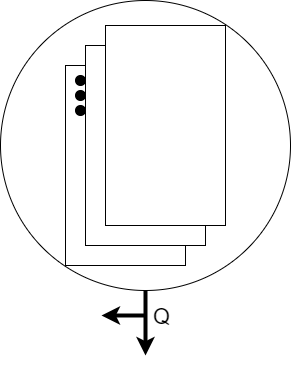
\includegraphics[width=.7\linewidth]{img/rechenberg_notation/auswahl_qualitaetsfunktion.png}
	\caption{Auswahl mit einer Qualitätsfunktion}
	\label{fig:auswahl_qualitaetsfunktion}
\end{subfigure}
\begin{subfigure}{.3\textwidth}
	\centering
	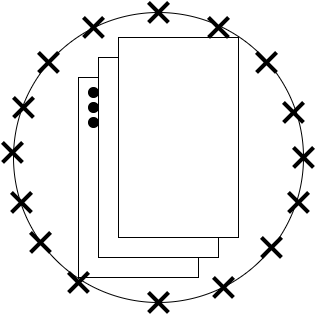
\includegraphics[width=.7\linewidth]{img/rechenberg_notation/population_isoliert.png}
	\caption{Isolierte Population}
	\label{fig:population_isoliert}
\end{subfigure}
\begin{subfigure}{.3\textwidth}
	\centering
	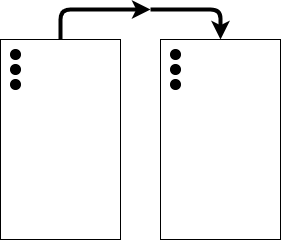
\includegraphics[width=.7\linewidth]{img/rechenberg_notation/duplikation.png}
	\caption{Duplikation}
	\label{fig:duplikation}
\end{subfigure}

\begin{subfigure}{.3\textwidth}
	\centering
	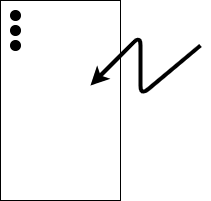
\includegraphics[width=.7\linewidth]{img/rechenberg_notation/mutation.png}
	\caption{Mutation}
	\label{fig:mutation}
\end{subfigure}
\begin{subfigure}{.3\textwidth}
	\centering
	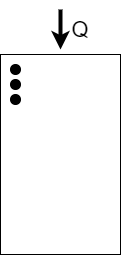
\includegraphics[width=.4\linewidth]{img/rechenberg_notation/bewertung.png}
	\caption{Bewertung}
	\label{fig:bewertung}
\end{subfigure}
\begin{subfigure}{.3\textwidth}
	\centering
	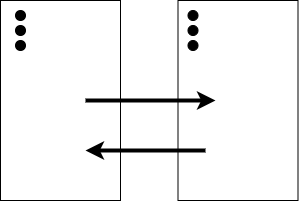
\includegraphics[width=.7\linewidth]{img/rechenberg_notation/rekombination.png}
	\caption{Rekombination}
	\label{fig:rekombination}
\end{subfigure}

\begin{subfigure}{.3\textwidth}
	\centering
	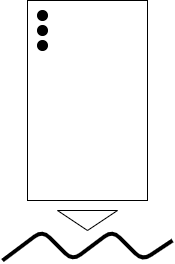
\includegraphics[width=.5\linewidth]{img/rechenberg_notation/phaenotypische_realisation.png}
	\caption{Phänotypische Realisation}
	\label{fig:phaenotypische_realisation}
\end{subfigure}
\caption{Rechenbergsche Grafik Notation}
\label{fig:rechenberg}
\end{figure}


% 3. Typische Reihenfolge der Abschnitte kurz zeigen. Aber auch klar machen das das ganze extrem variieren kann
